\newpage
%/\/\/\/\/\/\/\/\/\/\/\/\/\/\/\/\/\/\/\/\/\/\/\/\/\/\/\/\/\/\/\/\/\/\/\/\/\/\/\/\/\/\/\
\section{Sfere Soffici}\label{Soffici}
In un generico modello a \emph{Sfere Soffici} il potenziale di interazione tra le particelle è una funzione continua della distanze.
\newline
Il potenziale più adatto alla descrizione delle interazioni intermolecolari è quello proposto su base fenomenologica da Lennard-Jones, definito dall'equazione:
\begin{equation}
u(r) = 4\epsilon \biggr[\big(\frac{\sigma}{r} \big)^{12} - \big(\frac{\sigma}{r} \big)^6 \biggr]
\end{equation}
dove la costante $\epsilon$ rappresenta il minimo dell'energia e $\sigma$ la distanza di annullamento del potenziale.
\newline
I due esponenti sono stati scelti attraverso un criterio empirico, devono essere tali da determinare una forza di attrazione tra particelle distanti e una bariera repulsiva a distanze piccole.

	\begin{figure}[htbp]
		\centering
		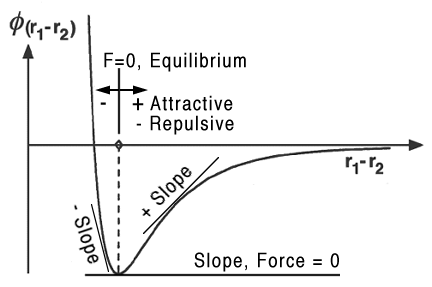
\includegraphics[scale=0.5]{Immagini/LJ}
		\caption[Potenziale di L.-J.]{Andamento del potenziale di Lennard-Jones.}\label{fig: LJunCut}
	\end{figure}




\FloatBarrier 
\subsection{Metodi Numerici e Simulazione Computazionale}
Come nel caso precedente, prima di passare allo studio del calcolo numerico della simulazione, è necessario scegliere un sistema di unità di misura caratteristico del modello.

\paragraph{Unità di Misura del sistema}
\begin{itemize}
\item[-] \underline{Massa}: $[M]=m=1$ 
\newline Tutte le particelle sono identiche è la loro massa fornisce l'unità di misura più ovvia.

\item[-] \underline{Lunghezza}: $[L]=\sigma=1$ 
\newline Il lato della scatola verrà genralmente misurato in unità di $\sigma$ (diametro della particella).

\item[-] \underline{Energia}: $[E]=\epsilon=1$ 
\newline Nell'espressione del potenziale è presente una scala naturale di energia data dalla costante $\epsilon$.
\end{itemize}
In queste unità di misura gli osservabili definiti nel capitolo (\ref{cap: Intro dinamica}) verrano espressi nel seguente modo:
\begin{eqnarray}
	\dfrac{kT}{\epsilon}  = T \\
	\dfrac{U}{N \epsilon} = U \\
	\dfrac{P \rho}{kT}	  = Z = 1 + P^{*}
\end{eqnarray}

\FloatBarrier 
\subsubsection{Taglio del potenziale}
Per simulare l'evoluzione del sistema è necessario conoscere la forza totale applicata su ogni particella che lo compone.
L'interazione tra sfere soffici è a 2 corpi e a lungo range, partanto sarà sarà necessario, in linea di pricipio, calcolare il contributo di interazione generato da ogni coppia di particelle, quindi $N(N-1)$ contributi in totale.

Come è visibile dalla figura (\ref{fig: LJunCut}, la forza diventa rapidamente molto piccola al crescere della distanza, si può quindi avere un notevole aumento nell'efficienza del calcolo trascurando le interazioni che avvengono a distanze troppo grandi.\newline
In altre parole è possibile considere un potenziale troncato del tipo:

\begin{displaymath}
	u_c(r) = 
	\begin{cases}u(r) & r \leq r_c\\
	0 & r > r_c \end{cases}
\end{displaymath}

Un potenziale di questa forma determina un troncamento anche per la forza associata con la conseguenza che 
ogni volta che una particella supera la distanza $r_c$ questa acquista un piccolo impulso.
Queste variazioni discontinue dei momenti determinano delle oscillazioni nell'energia totale del sistema annullando la conservazione dell'energia prevista per i sistemi isolati.

Quindi l'espressione troncata non rappresenta una buona approssimazione del potenziale iniziale.
E' necessario introdurre un'ulteriore correzione per assicurare la conservazione dell'energia definita dall'equazione:
\begin{equation}\label{eq: forza usata}
	F_{s}(r) = 
	\begin{cases}
	 -\dfrac{d}{dr} u(r) - \biggr(\dfrac{d}{dr} u(r)\biggr)\Biggr\vert_{r_c} & r \leq r_c\\
	0 & r > r_c 
	\end{cases}
\end{equation}
che determina un potenziale del tipo:
\begin{equation}\label{eq: potenziale usato}
	u_{s}(r) = 
	\begin{cases} u(r) - u(r_c) -[r -r_c]\biggr(\dfrac{d}{dr} u(r)\biggr)\Biggr\vert_{r_c} & r \leq r_c\\
	0 & r > r_c \end{cases}
\end{equation}
che sostanzialmente esprime una forza d'interazione troncata e traslata in modo da annullarsi alla distanza $r_c$.

L'andamento delle nuove espressioni della forza e dell'interazione è visibile nella figura (\ref{fig: LJCut}), dal grafico si può notare come la nuova forma alterata non sia estremamente simile dall'espressione iniziale.

	\begin{figure}[htbp]
		\centering
		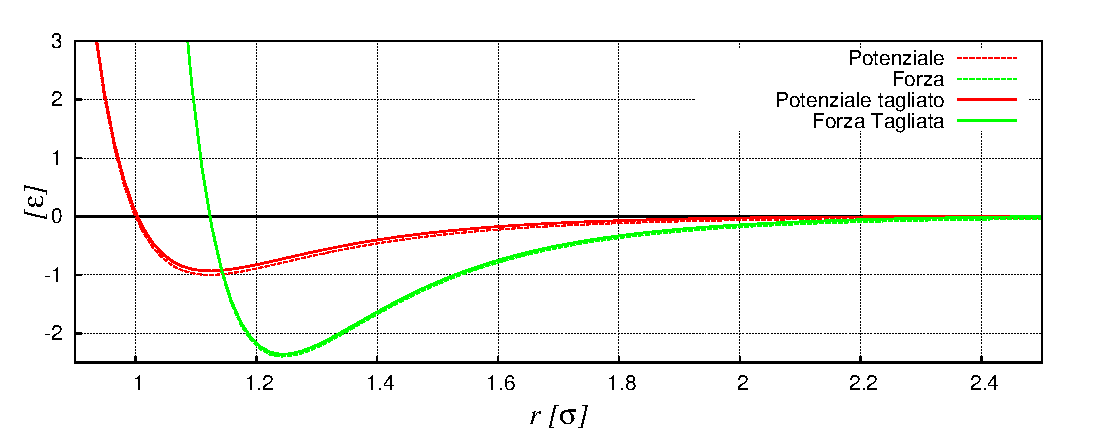
\includegraphics[scale=0.95]{Immagini/Soffici/potenziale}
		\caption[Potenziale di L.-J. tagliato]{Andamento del potenziale di Lennard-Jones tagliato e traslato e della forza corrispondente.}\label{fig: LJCut}
	\end{figure}

Tipicamente si sceglie come valore di taglio la distanza $r_c = 2.5 \sigma$ che corrisponde a trascurare valori della forza dell'ordine di $F(r_c) = -0.039 \epsilon / \sigma$.

\FloatBarrier 
\subsubsection{Metodo della lista dei vicini}
La parte della dinamica che richiede il maggiore sforzo computazionale è il calcolo della forza d'interazione, il metodo del potenziale troncato permette di migliorare l'efficienza di questa fase ma richiede in ogni caso di calcolare la distanza tra tutte le possibile coppie di particelle in ogni istante dell'evoluzione ( e in un sistema con bordo periodico tale misura non è immediata).

La velocità del calcolo numerico del sistema può essere ulteriormente raffinata introducendo la lista dei vicini.
Questa lista tiene conto di tutte le coppie di particelle che distano tra loro meno di $r_L \simeq r_c +0.3\sigma$, in questo funge da guida indicando quali coppie di particelle sono sufficientemente vicine da determinare una forza d'interazione non trascurabile.\newline
La distanza $r_L$ di "vicinanza" scelta è maggiore della distanza $r_c$ di "taglio", in questo modo la lista tiene traccia non solo delle particelle a distanza sufficientemente piccola da determinare un'interazione ma anche le particelle che entreranno nel raggio d'interazione in un certo intervallo di tempo $\check{T}$. \newline
Il vantaggio di tale prescrizione è di rendere la lista dei vicini valida per più di un evoluzione temporale, in tal caso non sarà necessario aggiornare la lista( e calcolare le distanze) ad ogni istante ma basterà farlo ogni $\check{T}$, intervallo di tempo pari a :
\begin{displaymath}
\check{T} \cdot \langle \vert \vec{v} \vert \rangle \simeq r_L - r_c = 0.3 \sigma
\end{displaymath}
corrispondende al tempo medio necessario ad una particella per percorrere la distanza $r_L - r_c$.

\FloatBarrier 
\subsubsection{Algoritmo di Evoluzione del sistema}
L'introduzione dell'espressione approssimata per l'interazione non altera le leggi che regolano l'evoluzione dinamica del sistema, restano, in ogni caso, da risolvere le equazioni differenziali del moto.
Per un sistema dotato di un grande numero di particelle come quello in esame la soluzione esatta del sistema di equazioni di Newton è totalmente improponibile.
L'unico approccio possibile è quello di affidarsi alle soluzione approssimate fornite dai metodi del calcolo numerico.

Esistono diversi metodi per il calcolo numerico delle soluzioni di equazioni differenziali, in generale nessuno di essi è in grado di calcolarla nel complesso ma solo di fornire una soluzione approssimata punto per punto risolvendo il problema di Cauchy su intervalli discreti consecutivi.
\newline
Pertanto sarà essenziale suddividere il tempo d'evoluzione in passi discreti, in questo articolo l'intervallo di tempo fondamentale è stato scelto pari a $t_{step} = 0.001 [t]$.
\medskip

L'algoritmo che è stato scelto per la simuluzione è il metodo di \emph{Velocity Verlet}( per il calcolo della soluzione delle equazioni del moto) che implementato congiuntamente alla tecnica della lista dei vicini determina il seguente ciclo per il calcolo del passo d'evoluzione del sistema:
\medskip
\begin{figure}[!htbp]
\begin{tikzpicture}[node distance = auto]
    % Place nodes
    \node [block_med] (1) {Evoluzione delle posizioni di ogni particella di un passo $\Delta t = t_{step}$ \newline \footnotesize $$\vec{r_i}(t_0) \mapsto \vec{r_i}(t_0 + \Delta t) = \vec{r_i}(t_0) + \vec{v_i}(t_0) \cdot \Delta t + \dfrac{1}{2} \vec{a_i}(t_0) \cdot \Delta t^2$$};
    \node [block_med, below of=1,node distance=2.25cm] (2) {Calcolo delle velocità a mezzo passo. \newline \footnotesize $$ \vec{v_i}(t_0 + \Delta t/2) = \vec{v_i}(t_0) + \dfrac{1}{2} \vec{a_i}(t_0) \cdot \Delta t$$ };
    \node [block_med, below of=2,node distance=2.55cm] (3) {Ricalcolo delle accelerazioni delle particelle. \newline \footnotesize $$\vec{a_i}(t_0) \mapsto \vec{a_i}(t_0 + \Delta t)=
     \overbrace{\sum_{i}^{} \sum_{j>i}^{}}^{j \in \text{Vicini}(i)} 
     F_s(\bar\vec{r_i}(t_0 + \Delta t) -\vec{r_j}(t_0 + \Delta t \bar )$$}; %\textrm($j$ vicino a $i$)    
    \node [decision, right of=3,node distance=9.25cm] (5) {\footnotesize Riaggiornamento della lista dei vicini ogni $10$ passi $\Delta t$.};        
    \node [block_med, below of=3,node distance=2.75cm] (4) {Evoluzione delle velocità in accordo con le accelerazioni aggiornate \newline \footnotesize $$\vec{v_i}(t_0) \mapsto \vec{v_i}(t_0 + \Delta t) = \vec{v_i}(t_0 + \Delta t/2) + \dfrac{1}{2}\vec{a_i}(t_0+\Delta t)\cdot \Delta t$$};
 
    % Draw edges
    \path [line] (1) -- (2);
    \path [line] (2) -- (3);
    \path [line] (3) -- (4);
    \path [line] (4) -| (5);
    \path [line] (5) |- (1);
\end{tikzpicture}
\end{figure}

\FloatBarrier 
\subsubsection{Implementazione computazionale dell'algoritmo}
Per simulare questo sistema verrà utilizzata la programmazione ad oggetti del linguaggio C++.
La logica usata per il programma è la stessa sfrutta per la simulazione del sistema a sfere rigide.
\newline
Si definire la classe \Cls{sistema\_soffice()} dotata degli attributi necessari a descrivere lo stato microscopico del sistema:
\begin{itemize}
\item 3 array di vettori per memorizzare posizione, velocità e accelerazione di tutte le particelle costituenti il sistema.

\item 2 array per memorizzare la \emph{lista dei vicini} associata allo stato del sistema. Il vettore \cd{NPoint} contiene nell'ingresso $i$ l'indice del vettore \cd{List} dopo di cui comincia l'elenco delle particelle vicine alla particella $i$. Il vettore \cd{List} viene costruito testando in modo sequenziale tutte le coppie $($ $P[i]$, $P[j]$ $)_{j>i}$ e salvando tutti gli indici $j$ relativi a coppie "vicine" secondo la definizione del paragrafo precedente.

\item 5 variabili \emph{double} per contenere le variabili $r_c$, $r_L$,$\sigma$,$\epsilon$ e L. 2 varibili \emph{int} per salvare il numero di particelle e la dimensione spaziale della simulazione.

\end{itemize}
%\medskip\newline
Il costruttore della classe costituirà la fase di \emph{inizializzazione} dell'algoritmo, ovvero salverà le posizioni disponendole nel reticolo bcc più piccolo in grando di contenerle tutte, attribuirà velocità iniziali casuali riscalandole a Momento totale nullo, inizializza la lista dei vicini e calcola le accelerazioni per la prima volta.
Le variabili necessarie per inizializzare il sistema, argomenti della funzione costruttore, saranno la dimensione spaziale $d$, la densità del sistema e il numero $N$ di particelle contenute.
\medskip\newline
Il metodo \cd{evoluzione()} è il cardine della simulazione, questa funzione fornisce l'evoluzione temporale del sistema di un $t_{step}$ sfruttando la tavola dei vicini precedentemente calcolata. I metodi che calcolano passi d'evoluzione consecutivi provvederanno a ricalcolare la lista dei vicini ogni 10 $t_{step}$
\medskip\newline
La fase di \emph{termalizzazione} si ottiene applicando il metodo di evoluzione un numero di volte sufficiente a realizzare la distribuzione di Maxwell-Boltzman per le velocità.
\medskip\newline
Similmente la fase di \emph{produzione} si realizza intervallando la raccolta di osservabili istantanei sulla configurazione occupata dal sistema all'evoluzione temporale necessaria per ottenere un'altra configurazione sufficientemente scorrelata dalla prima.
\medskip\newline
Per ottenere rapidamente una successione di sistemi inizializzati con un diverso numero di particelle e valore di densità viene usato il metodo \cd{rinizializzazione()}. Tale metodo prende in ingresso i nuovi valore di $N$ e di $rho$ (minori di quelli precedenti), ricalcola il lato della scatola, espande proporzionalmente i vettori posizione e ricalcola la lista dei vicini di conseguenza.



\FloatBarrier 
\subsection{Caratteristiche dell'algoritmo di Simulazione}
\begin{figure}[htbp]
		\caption[Sfere Soffici$/$Preliminari\_Snap2D.cpp]{Immagini del sistema 2D termalizzato a diversi valori di densità e Temperatura (In alto a sinistra è visibile la configurazione inziale prima dell'evoluzione temporale).}\vspace{-15pt}
        \begin{subfigure}[b]{0.5\textwidth}
                \centering
                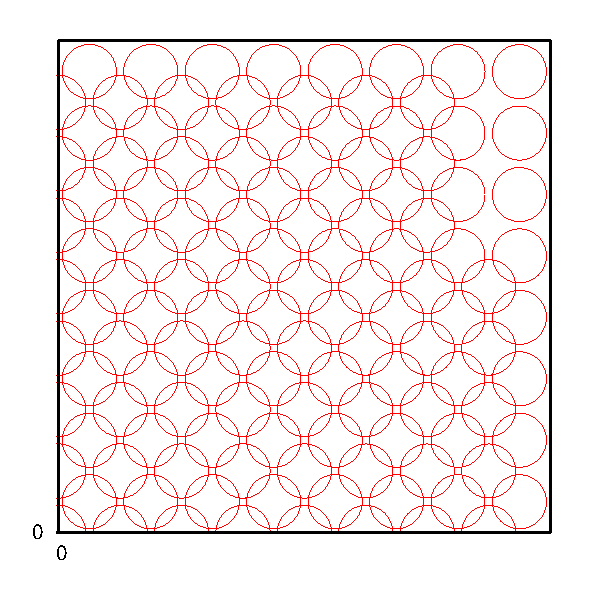
\includegraphics[width=0.85\textwidth]{Immagini/Soffici/SnapSolidoCompresso_Inizio_2D}
        \end{subfigure}%
        ~ %add desired spacing between images, e. g. ~, \quad, \qquad etc. 
          %(or a blank line to force the subfigure onto a new line)
        \begin{subfigure}[b]{0.5\textwidth}
                \centering
                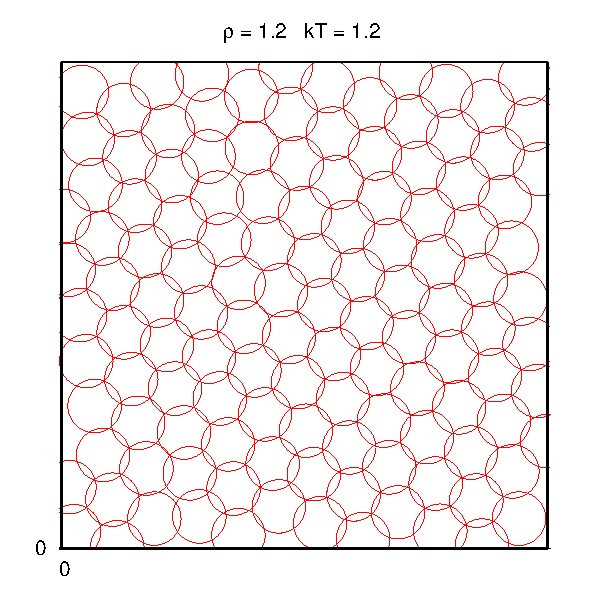
\includegraphics[width=0.85\textwidth]{Immagini/Soffici/SnapSolidoCompresso_2D}
        \end{subfigure}
        ~ %add desired spacing between images, e. g. ~, \quad, \qquad etc. 
          %(or a blank line to force the subfigure onto a new line)

        \begin{subfigure}[b]{0.5\textwidth}
                \centering
                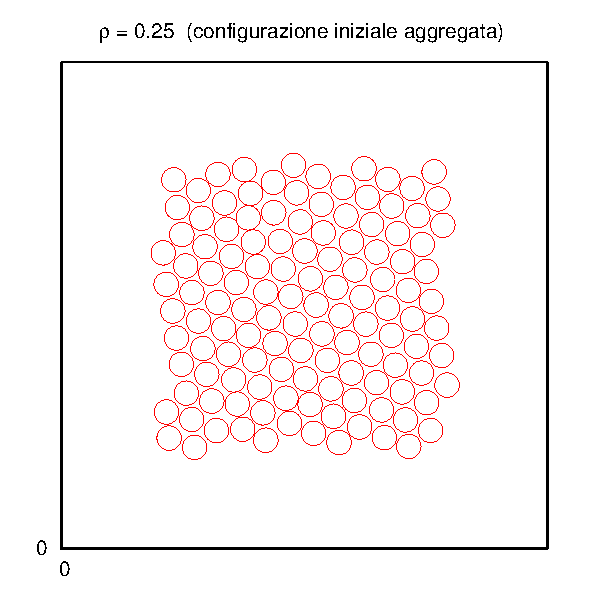
\includegraphics[width=0.85\textwidth]{Immagini/Soffici/SnapSolidoFreddo_Inizio_2D}
        \end{subfigure}
         \begin{subfigure}[b]{0.5\textwidth}
                \centering
                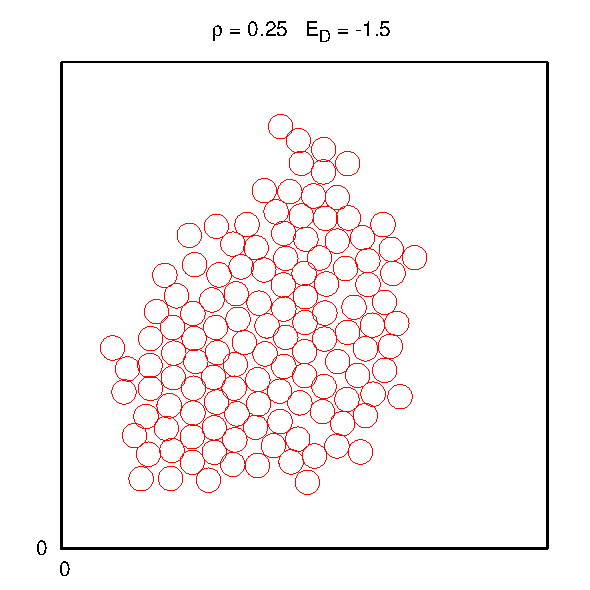
\includegraphics[width=0.85\textwidth]{Immagini/Soffici/SnapSolidoFreddo_2D}
        \end{subfigure}
		
        \begin{subfigure}[b]{0.5\textwidth}
                \centering
                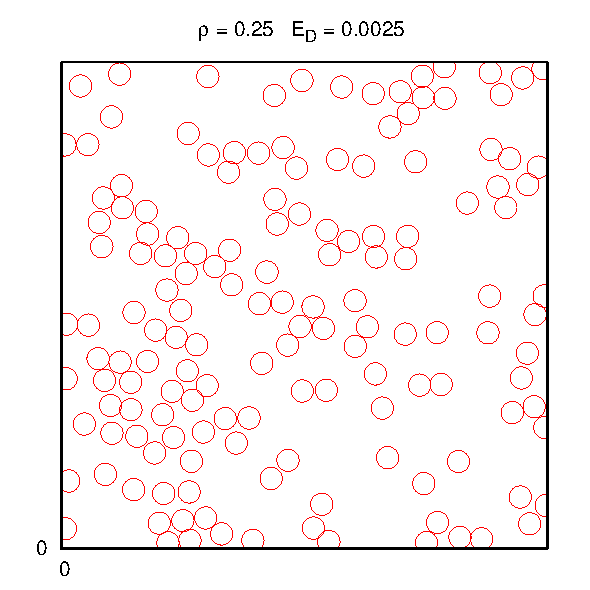
\includegraphics[width=0.85\textwidth]{Immagini/Soffici/SnapSolidoFreddo_2D_Nuclea}
        \end{subfigure}
         \begin{subfigure}[b]{0.5\textwidth}
                \centering
                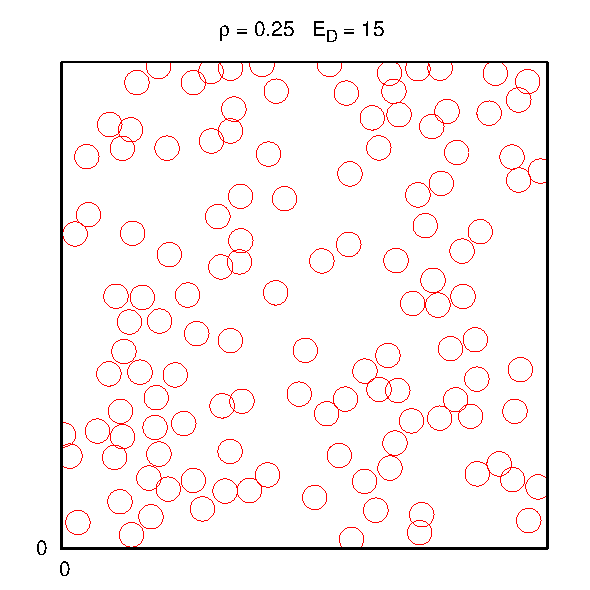
\includegraphics[width=0.85\textwidth]{Immagini/Soffici/SnapLiquido_2D}
        \end{subfigure}
		
		 \centering  \footnotesize{$N= 125$ , $d=2$ , N passi Termalizzazione =$ 500000 $}
		\label{fig: snap2d_soft}
\end{figure}
Nella figura (\ref{fig: snap2d_soft}) sono mostrate delle istantantanee delle configurazioni del sistema a sfere soffici termalizzato a diversi valori delle variabili Termodinamiche che certificano la presenza di una transizione di fase solido-liquido anche per questo modello.
Similmente a quanto accadeva per le sfere rigide il sistema presenta un congelamento di natura geometrica infatti per elevati valori di densità le molecole sono vincolate in un reticolo regolare per via della divergenza infinita del potenziale a brevi distanze (prime 2 figure).

Se l'energia media delle particelle è sufficientemente bassa, la presenza di forze attrattive determina la solidificazione del sistema anche in condizioni di bassa densità.
L'algoritmo usato per la termalizzazione, che consiste in una successione di passi evolutivi intervallati dal riscalamento delle velocità del sistema ad un valore di temperatura( quindi energia cinetica) controllato, non è il procedimento ideale per mostrare questo tipo di transizione.
Nel caso in cui si cerchi di far solidificare un sistema molto rarefatto saranno necessari numerosi passi evolutivi affinchè le particelle, estremamente rallentate dall'abbassamento di temperatura, riescano ad avvicinarsi a sufficienza da aggregarsi e dare il via alla nucleazione.

L'immagine ottenuta precedentemente( ultime 4 figure) invece è stata realizzata a partire da una configurazione ordinata posta in un volume ampio( in modo da diminuire la densità totale), non è in grado di mostrare la solidificazione ma dimostra come il sistema rimanga aggregato in un regione densa in condizione di bassa temperatura sofficiente da non permettere alle molecole di fuoriuscire dai pozzi di potenziale generati dalla sovrapposizione di tutte le interazioni.
La simulazione riesce però a mostrare corrattamente l'evaporazione di questa struttura densa con il riscaldamento del sistema.

\FloatBarrier 
\subsubsection{Tempo di esecuzione}
Il parametro principale che regola il tempo macchina richiesto dalla simulazione di un singolo step di evoluzione del sistema è la dimensione della lista dei vicini. 
Tale lunghezza dipende principalmente da 3 parametri( specifici della simulazione) il numero $N$ di particelle, la densità del sistema $\rho$ e la dimensione spaziale $d$.
Nelle figure (\ref{fig: T_Esec_Confronto_D Soffici}) e (\ref{fig: T_Esec_Confronto_rho Soffici}) è mostrato l'andamento del tempo di esecuzione medio di uno step evolutivo in fuzione del numero $N$ di particelle simulate e per vari valori di densità $\rho$.

	\begin{figure}[htbp]
		\centering
		\caption[Sfere Soffici$/$Preliminari\_TempoEsecuzione.cpp]{Andamento del tempo di esecuzione in funzione del numero di particelle simulate e della Dimensione Spaziale.}\label{fig: T_Esec_Confronto_D Soffici}\vspace{-15pt}
		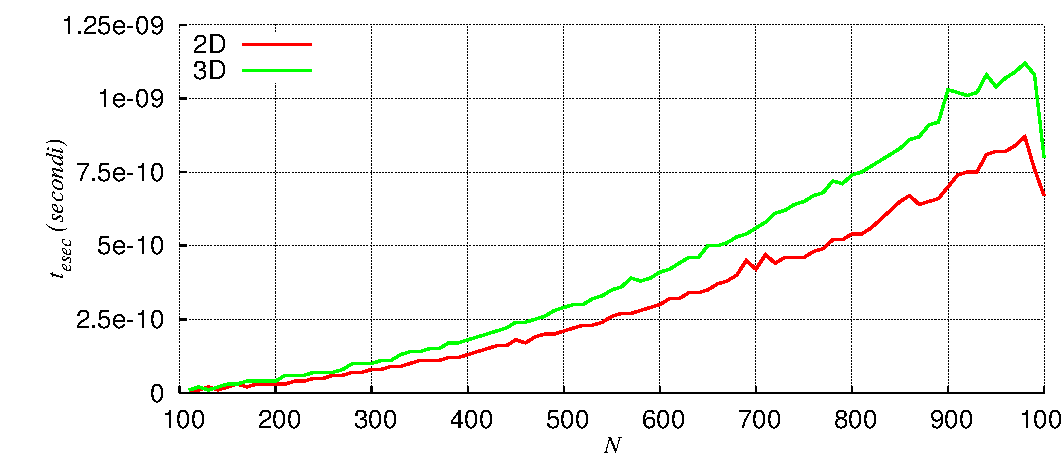
\includegraphics[scale=0.85]{Immagini/Soffici/TempoEsecuzione_ConfrontoD}

		\centering  \footnotesize{$\rho=0.8$ , Media su $ 1000000 $ passi}
	\end{figure}

Ovviamente si osserva un aumento del tempo-macchina con la crescita del numero di particelle simulate, questo determina un maggior numero test da effettuare per determinare la vicinanza tra le coppie .
\newline
D'altro canto una desità molto alta implica che le particelle siano statisticamente molto vicine tra loro, quindi, a parità del numero delle molecole, andranno calcolate in medeia le interazioni su un maggior numero di punti. Nella figura (\ref{fig: T_Esec_Confronto_rho Soffici}) è possibile osservare questo effetto.
\newline
La dimensionalità dello spazio influisce invece sul "impaccamento" delle particelle (soprattutto nelle configurazioni particolarmente dense). Ad esempio una sfera in uno spazio 3-dimensionale potrà venire a contatto con un maggiore numero di sfere sulla sua superficie rispetto ad un cerchio (quindi in 2 dimensioni) dello stesso raggio sulla sua superficie.
Il confronto tra i tempi di esecuzione tra  sistemi di dimensione diversa ma di pari densità è mostrato nella figura (\ref{fig: T_Esec_Confronto_D Soffici}).

	\begin{figure}[htbp]
		\centering
		\caption[Sfere Soffici$/$Preliminari\_TempoEsecuzione.cpp]{Confronto tra l'andamento del tempo di esecuzione a vari valori di densità del sistema.}\label{fig: T_Esec_Confronto_rho Soffici}\vspace{-15pt}
		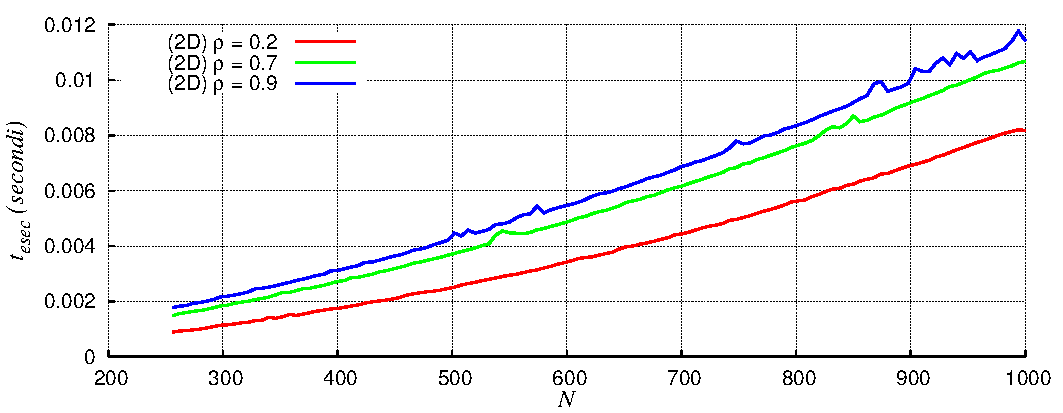
\includegraphics[scale=0.85]{Immagini/Soffici/TempoEsecuzione2D}

		\centering  \footnotesize{$d=2$ , Media su $ 50000 $ passi}
	\end{figure}


\FloatBarrier 
\subsubsection{Tempo di Termalizzazione}
In questo sistema è possibile definire due diversi processi di termalizzazione: nel primo si interviene fissando l'energia meccanica totale del sistema mentre nel seconda si fissa la temperatura del sistema, quindi solo l'enegia cinetica media.
Siccome le due quantità sono di natura differente, una è puramente istantanea e costantemente conservata mentre l'altra è una quantità soggetta a fluttuazioni termiche, lo studio del tempo di termalizzazione va effettuato in modo separato.

	\begin{figure}[htbp]
		\centering
		\caption[Sfere Soffici$/$Preliminari\_Termalizzazione.cpp]{Andamento degli osservabili istantanei in funzione del numero di passi d'evoluzione per vari valori di densità}\label{fig: Termal E D Soffici}\vspace{-15pt}

		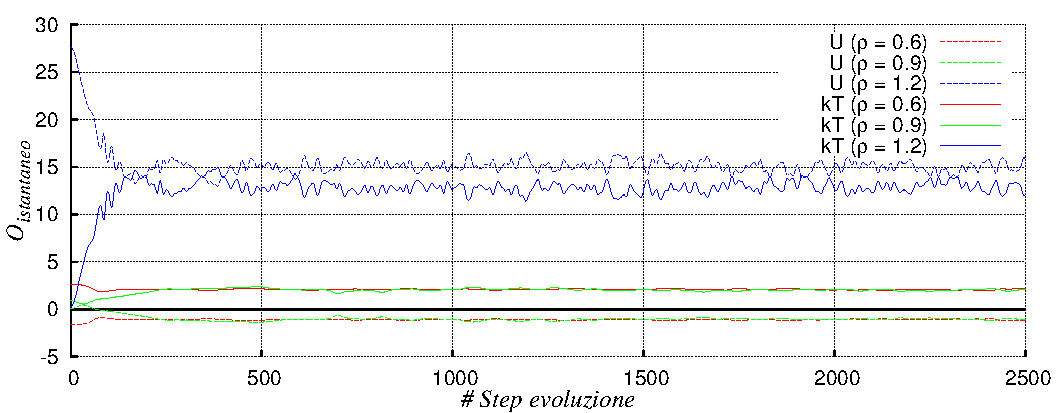
\includegraphics[scale=0.95]{Immagini/Soffici/Termal_OvsStep}

		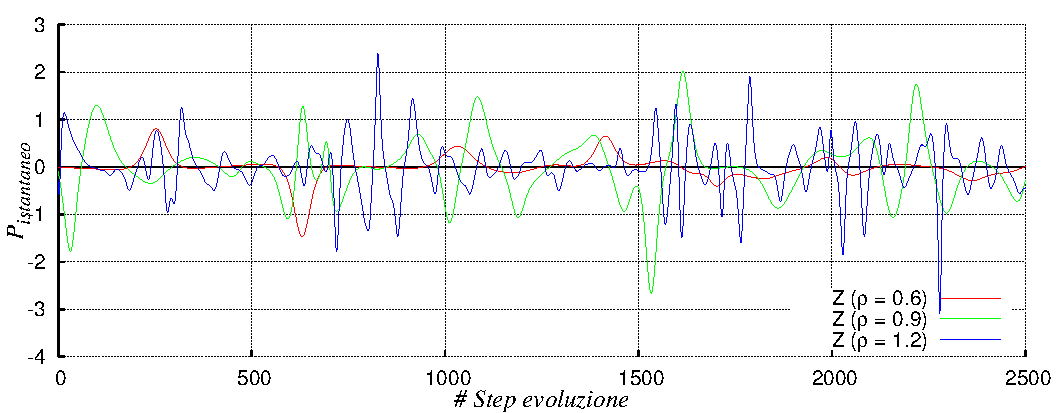
\includegraphics[scale=0.95]{Immagini/Soffici/Termal_PvsStep}

		\centering  \footnotesize{$N= 250$ , $d=3$ , $E_D$ per particella =1}
	\end{figure}
	
Il tempo di termalizzazione ad Energia definita si può studiare osservando l'andamento degli osservabili istantanei in funzione del numero di step di evoluzione, quando i valori tendono ad oscillare intorno ad un valore medio si può considerare raggiunta la condizione di termalizzazione. 
Secondo la figura (\ref{fig: Termal E D Soffici}) , dove è mostrato l'andamento di $P*$,$kT$ e$U$ in funzione del numero di passi di evoluzione, $500$ step sarebbero sufficienti a portare a termalizzazione un sistema di $250$ particelle.
\medskip\newline
Nel caso della termalizzazione a $kT$ definito, invece, è possibile sfruttare la funzione $H$ di Boltzman per valutare il tempo di termalizzazione.

	\begin{figure}[!htbp]
		\centering
		\caption[Sfere Soffici$/$Preliminari\_Termalizzazione.cpp]{Andamento dei valori della funzione di Boltzman in funzione del numero di passi d'evoluzione per vari valori di densità}\label{fig: Termal H T_D Soffici}\vspace{-15pt}
		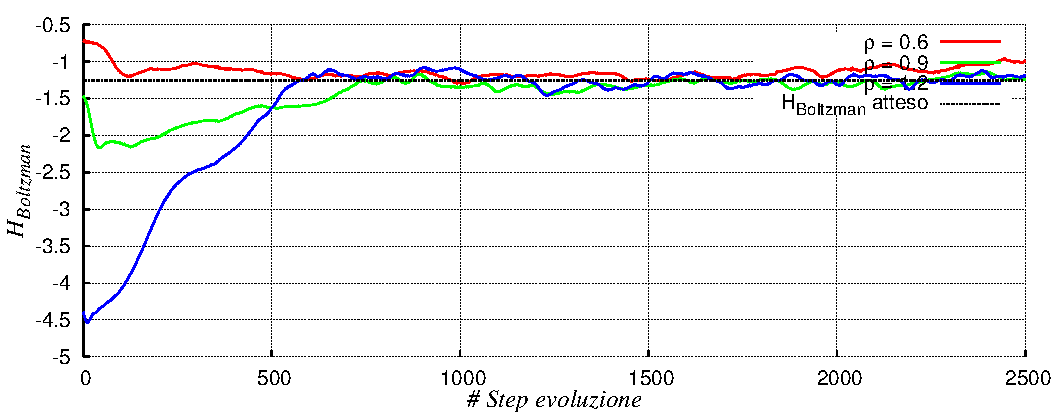
\includegraphics[scale=0.95]{Immagini/Soffici/Termal_HvsStep}

		\centering  \footnotesize{$N= 250$ , $d=3$ , $H$ media calcolata ogni 5 passi}
	\end{figure}
	
Nella figura (\ref{fig: Termal H T_D Soffici}) è mostrato l'andamento della funzione $H$ calcolata su $25$ configurazioni successive campionate dopo una termalizzazione a temperatura costante ( $kT=1$ ) effettuata per $n$ passi evolutivi a partire dal reticolo $BCC$ iniziale.
Dal grafico si può nota come i valori campionati comincino ad oscillare attorno al valore atteso dopo circa $1000$ evoluzioni, la statistica raccolta in un singolo istante non è sufficientemente ampia da poter approssimare l'istogramma delle componenti delle velocità alla loro effettiva distribuzione, in questo caso l'accordo completo non è mai raggiungibile.

	\begin{figure}[!htbp]
		\centering
		\caption[Sfere Soffici$/$Preliminari\_Termalizzazione.cpp]{Istogramma della distribuzione dei valori delle componenti x delle velocità raccolte dopo la termalizzazione}\label{fig: Termal Isto T_D Soffici}\vspace{-15pt}
		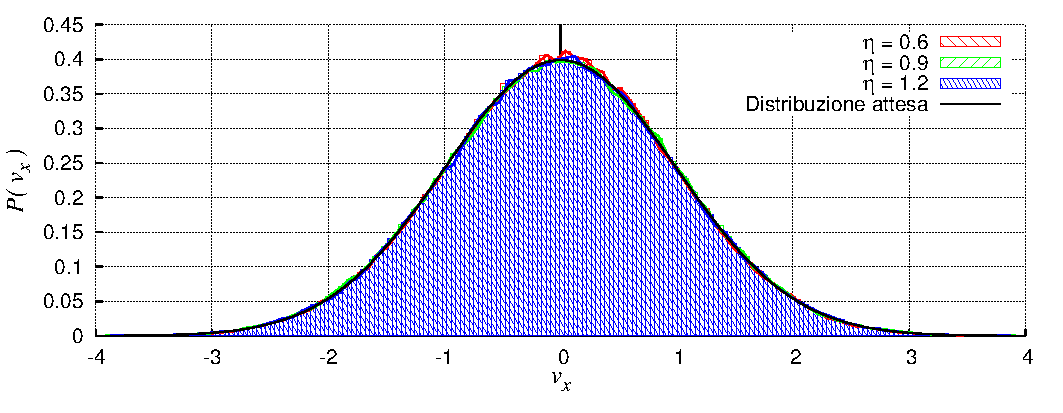
\includegraphics[scale=0.95]{Immagini/Soffici/DistroVx}

		\centering  \footnotesize{$N= 250$ , $d=3$ , N passi Termalizzazione =$ 5000$, $T_D=1$, intervallo di campionamento 50 step.}
	\end{figure}
	
Aumentando il numero di configurazioni campionate risulta, a seguito della termalizzazione precedente, la distribuzione di probabilità visibile in figura (\ref{fig: Termal Isto T_D Soffici}), che mostra un ottimo accordo con la distribuzione gaussiana prevista per la temperatura prescelta.


\FloatBarrier 
\subsection{Caratteristiche del modello, studio delle transizioni di fase}
In questo caso la determinazione della transizione di fase attraverso lo studio dell'andamento di un parametro d'ordine, quale Z, $ds^2$ o il numero medio di particelle vicini, è leggermente più impegnativa rispetto al modello precedente.

Il motivo di questa complicazione è da ricercare nella dipendenza dello stato non più dal solo parametro $\rho$ ma anche da $T_D$ che nel modello a sfere rigide era  una variabile fissata il cui valore determinava solamente un riscalamento dell'unità di tempo.
Per determinare la transizione di fase sarebbe necessario realizzare un grafico 3 dimensionale del parametro d'ordine in funzione delle due variabili di stato indipendenti. Tale procedimento è computazionalmente molto lungo in quanto richiederebbe il calcolo di troppi punti per ottenere una buona risoluzione, pertanto l'analisi della transizione di fase si limita allo studio della diffusione.


\subsubsection{Andamento delle Oscillazioni Termiche}
In un sistema conservativo l'energia meccanica totale è costantemente conservata ma in presenza, come in questo caso,  di un potenziale non nullo, non sono le singole componenti dell'energia ad essere conservate ma sono presenti continui scambi tra la componente interna e quella cinetica.
Nella figura (\ref{fig: Problema9}) è mostrata l'andamento della densità di energia interna istantanea, in un sistema già termalizzato, per due casi con diverso numero di particelle.

	\begin{figure}[htbp]
		\centering
		\caption[Sfere Soffici$/$Problema9.cpp]{Andamento dei valori della densità di energia interna istantanea in funzione del tempo di evoluzione a seguito della termalizzazione.}\label{fig: Problema9}\vspace{-15pt}

		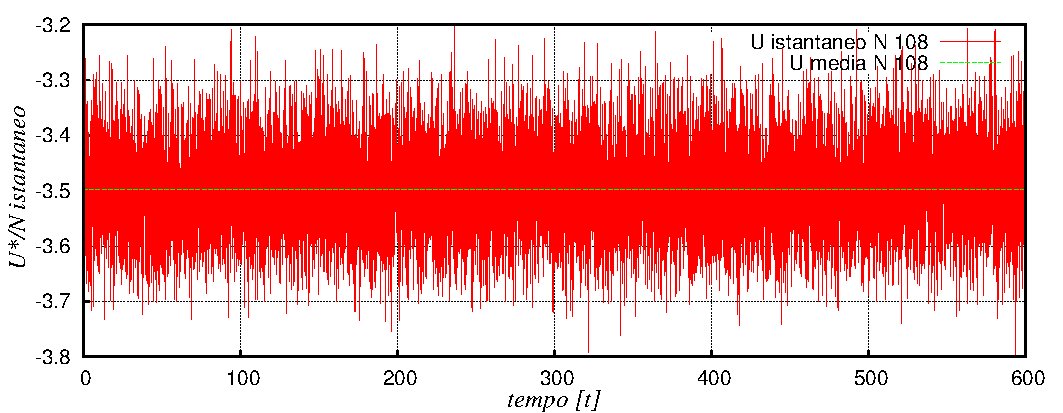
\includegraphics[scale=0.75]{Immagini/Soffici/UvsStepN108}

		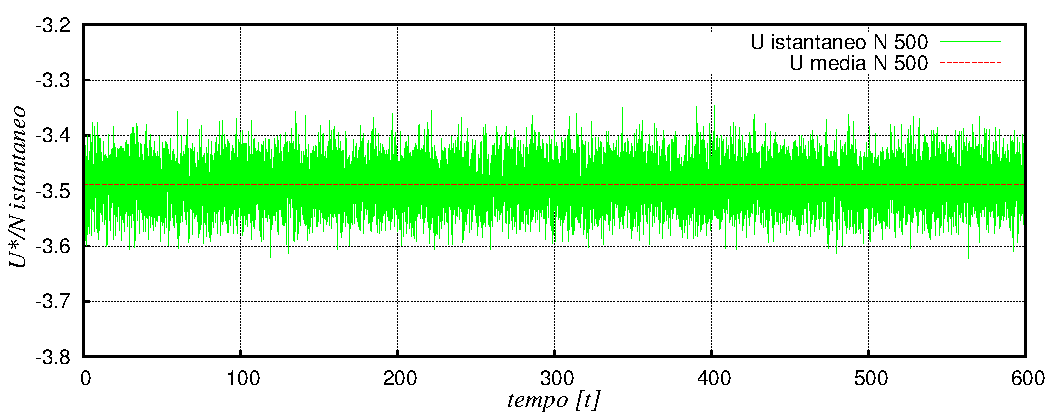
\includegraphics[scale=0.75]{Immagini/Soffici/UvsStepN500}

		\centering  \footnotesize{$N= 250$ , $d=3$ , N passi Termalizzazione =$ 5000$, $\rho = 0.7$,	$T_D=1.19$, campionamento ogni $0.015 [t]$.}
	\end{figure}

E' evidente come l'ampiezza delle fluttuazioni decresca all'aumentare del numero di molecole simulate (per conferma è stato realizzato nella figura (\ref{fig: Isto_Problema9}) l'istogramma dei valori istantanei raccolti), ci si aspetta che nel limite termodinamico tale quantità possa essere considerata una costante per un sistema in equilibrio.

	\begin{figure}[htbp]
			\centering
		\caption[Sfere Soffici$/$Problema9.cpp]{Istogramma dei valori campionati per la figura precedente.}\label{fig: Isto_Problema9}\vspace{-15pt}

		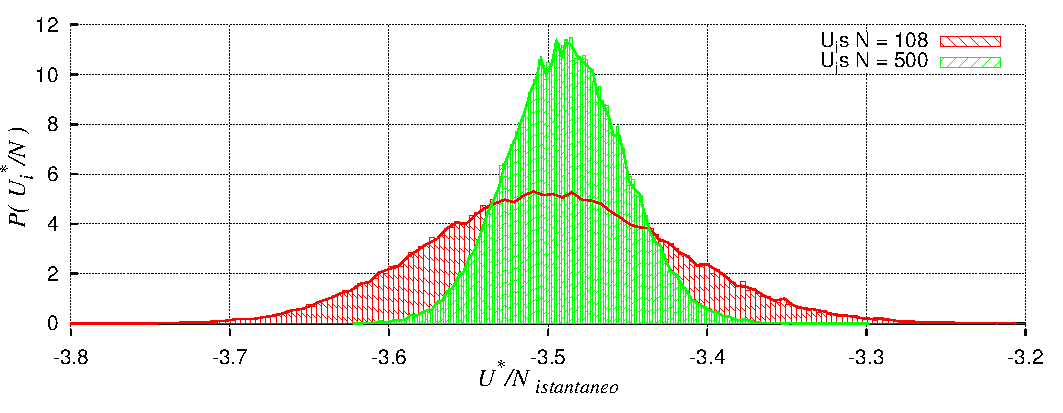
\includegraphics[scale=0.85]{Immagini/Soffici/IstoU}

	\end{figure}
	
Nella figura (\ref{fig: Problema10}) viene comparato l'andamento dei 3 osservabili istantanei in funzioni dei passi evolutivi. La prima prima cosa che si può notare è come la temperatura, legata all'energia cinetica media, oscilli in senso opposto rispetto alla densità di energia interna. L'effetto è dovuto alla conservazione dell'energia totale che obbliga le fluttuazioni ad annullarsi.
In secondo luogo, analizzando l'istogramma, si osserva che le oscillazione dell'osservabile $P*$ sono molto più ampie rispetto a quelle degli altri due.
	
	\begin{figure}[htbp]
		\centering
		\caption[Sfere Soffici$/$Problema10.cpp]{Andamento delle osservabili istantanee della simulazione in funzione del tempo di evoluzione a seguito della termalizzazione.}\label{fig: Problema10}\vspace{-15pt}
		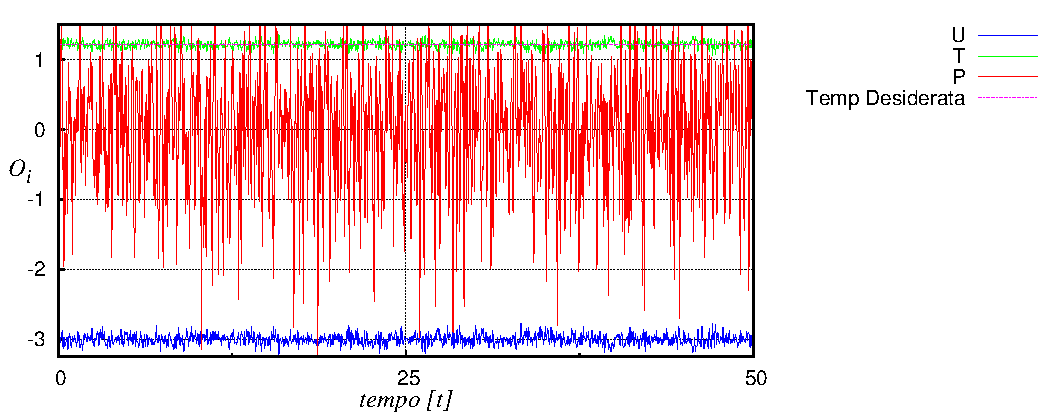
\includegraphics[scale=0.85]{Immagini/Soffici/OvsStep}

		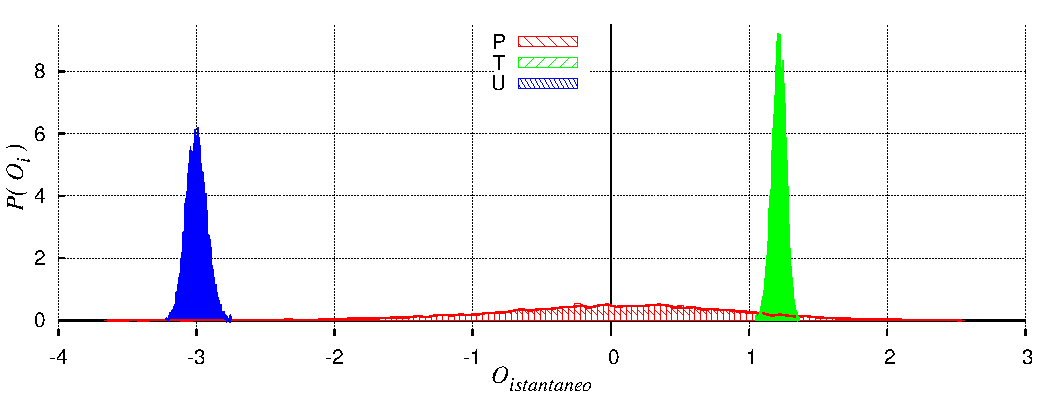
\includegraphics[scale=0.85]{Immagini/Soffici/IstoO}


		\centering  \footnotesize{$N= 108$ , $d=3$ , N passi Termalizzazione =$ 5000$, $\rho = 0.6$,	$T_D=1.22$, campionamento ogni $0.015 [t]$.}
	\end{figure}



\FloatBarrier 
\subsubsection{Studio della Diffusione: Spostamento Quadratico Medio e Funzione di Distribuzione Radiale}
Si procede ora allo studio della diffusione per determinare la fase fisica del sistema come spiegato nel capitolo introduttivo.

Nel grafico (\ref{fig: Problema11}) è mostrato l'andamento dello spostamento quadratico medio (calcolato senza bordo) in fuzione del tempo per lo stesso sistema a diverse temperature.
	\begin{figure}[htbp]
		\centering
		\caption[Sfere Soffici$/$Problema11.cpp]{Andamento dello spostamento quadratico medio in funzione del tempo di diffusione per vari valori di temperatura}\label{fig: Problema11}\vspace{-15pt}

		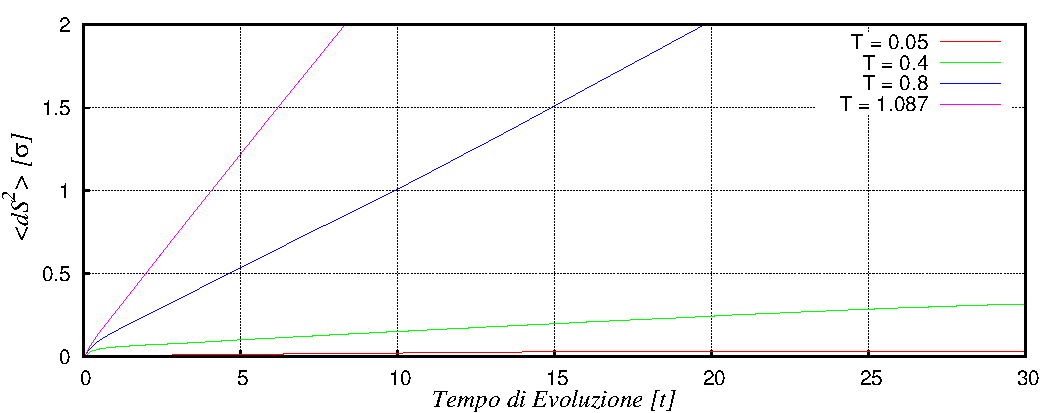
\includegraphics[scale=0.95]{Immagini/Soffici/dS_quadvsDt}

		\centering  \footnotesize{$N= 256$ , $d=3$ , N passi Termalizzazione =$ 10000$, $\rho = 0.9$, $\#$ campionature = $ 4000$, campionamento ogni $0.015 [t]$.}
	\end{figure}
Le simulazioni sono ottenute in modo consecutivo partendo dalla temperatura più bassa e termalizzando a temperature crescente per ottenere i diversi andamenti.


	\begin{figure}[htbp]
		\centering
		\caption[Sfere Soffici$/$Problema11$\_$v2C.cpp]{Funzione di distribuzione radiale $g_t(r)$ a vari valori di densità e temperatura alta.}\label{fig: Problema11_v2C}\vspace{-15pt}

		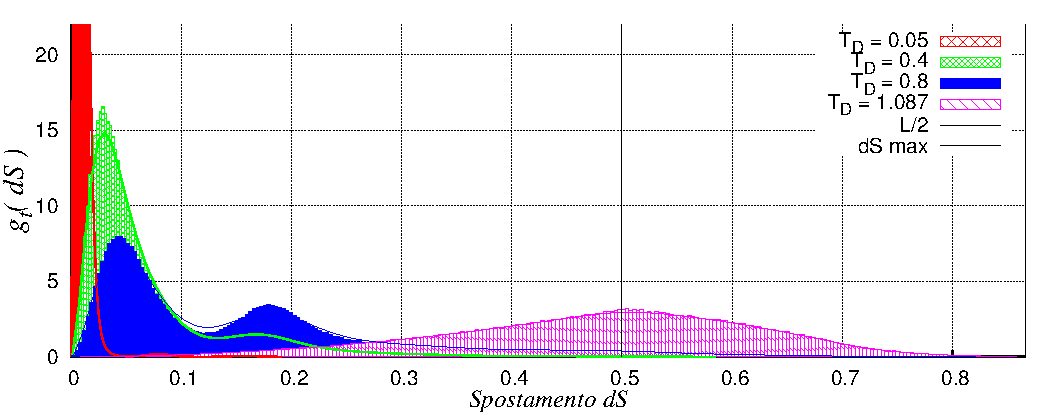
\includegraphics[scale=0.95]{Immagini/Soffici/DistrodS_RhoAlta_3D}
		
		\centering  \footnotesize{$N= 256$ , $d=3$ , N passi Termalizzazione =$ 10000$, $\rho = 0.9$, $\#$ campionature = $ 4000$,\newline $\Delta t = 0.015 [t] = 15 t_{step}$, intervallo di tempo tra ogni campionamento = 10 $\Delta t$, tempo di diffusione = 3000 $\Delta t$}
	\end{figure}
Calcolando la funzione di distribuzione radiale  per gli stessi sistemi si ottiene la figura (\ref{fig: Problema11_v2C}). E' evidente come alla temperatura $T=1.087$ il sistema si trovi in una fase liquida  mentre per la temperatura più bassa ($T=0.8$) sviluppi una struttura solida metastabile. In quest'ultimo caso sono visibili due picchi compatibili con la presenza simultanea di un nucleo denso localizzato, in grado di tratenere le particelle più lente, e un gas di particelle più veloci che riescono ad evaporare dall' aggregato congelato.
\medskip

Confrontando il sistema precedente con una simulazione dello stesso tipo ma a densità minore si può notare come la temperatura di cambiamento di fase sia determinata dalla velocità.
	\begin{figure}[htbp]
		\centering
		\caption[Sfere Soffici$/$Problema11$\_$v2B.cpp]{Funzione di distribuzione radiale $g_t(r)$ a vari valori di temperatura a partire dalla configurazione iniziale congelata a bassa densità.}\label{fig: Problema11_v2B}\vspace{-15pt}

		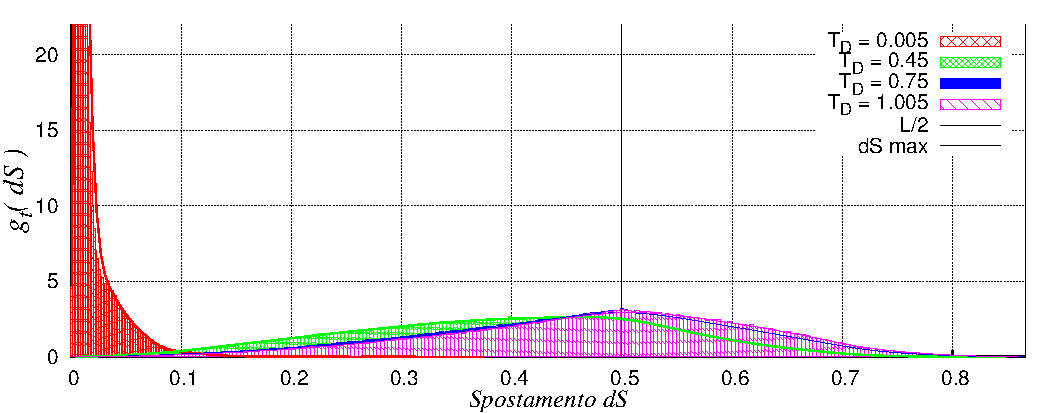
\includegraphics[scale=0.95]{Immagini/Soffici/DistrodS_RhoBassa_3D}

		\centering  \footnotesize{$N= 256$ , $d=3$ , N passi Termalizzazione =$ 10000$, $\rho = 0.25$, $\#$ campionature = $ 2000$,\newline $\Delta t = 0.05 [t] = 15 t_{step}$, intervallo di tempo tra ogni campionamento = 10 $\Delta t$, tempo di diffusione = 3000 $\Delta t$}
	\end{figure}
Nella figura (\ref{fig: Problema11_v2B}), in cui è rappresenatata la funzione di distribuzione radiale per un sistemà a densità  $\rho = 0.25$, si può notare come a temperature simili alla fase solida metastabile del sistema precedente il sistema a bassa densità si trovi già allo stato liquido. In questo caso, per eliminare il tempo  di evoluzione necessario al configurazione in disposizione $BCC$ di nucleare, il sistema è stato inizializzato già aggregato.

\medskip

Può essere interessante studiare la funzione $g_t(r)$ anche per sistema alla stessa temperatura ma con diversa densità.
Nella figura (\ref{fig: Problema11_v2A}) sono mostrati tali andamenti, si può vedere come il sistema possa termalizzarsi in uno stato solido anche a temperature alte se la densità è sufficientemente elevata.
	\begin{figure}[htbp]
		\centering
		\caption[Sfere Soffici$/$Problema11$\_$v2A.cpp]{Funzione di distribuzione radiale $g_t(r)$ a vari valori di densità e temperatura fissata.}\label{fig: Problema11_v2A}\vspace{-15pt}

		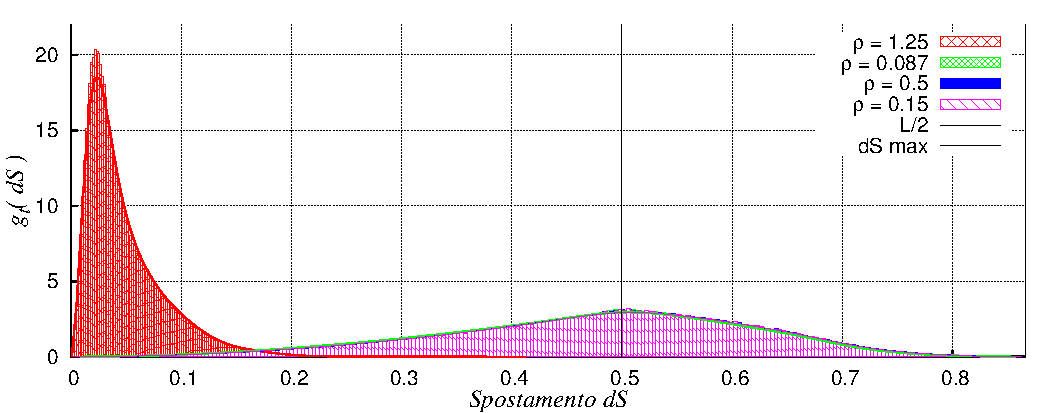
\includegraphics[scale=0.95]{Immagini/Soffici/DistrodS_Rho_3D}
		
		\centering  \footnotesize{$N= 256$ , $d=3$ , N passi Termalizzazione =$ 10000$, $T_D = 0.9$, $\#$ campionature = $ 2000$,\newline $\Delta t = 0.05 [t] = 15 t_{step}$, intervallo di tempo tra ogni campionamento = 10 $\Delta t$, tempo di diffusione = $3000 Delta t$}
	\end{figure}



\FloatBarrier 
\subsection{Studio del limite termodinamico}
Si procede ora alla stima dei variabili di stato di un sistema al limite termodinamico. Nella figura (\ref{fig: Limite Termo}) è mostrato il valore di $\langle Z-1 \rangle$  calcolato per sistemi caratterizzati dalla stessa densità ed energia molecolare media ma simulati con diverso numero di particelle.

\begin{figure}[htbp]
\centering
	\caption[Sfere Soffici$/$Problema12.cpp $\quad \rightarrow \quad$ ZvsN\_file.p]{Andamento del parametro Z-1 in funzione di $N$. Limite Termodinamico }\vspace{-15pt}
	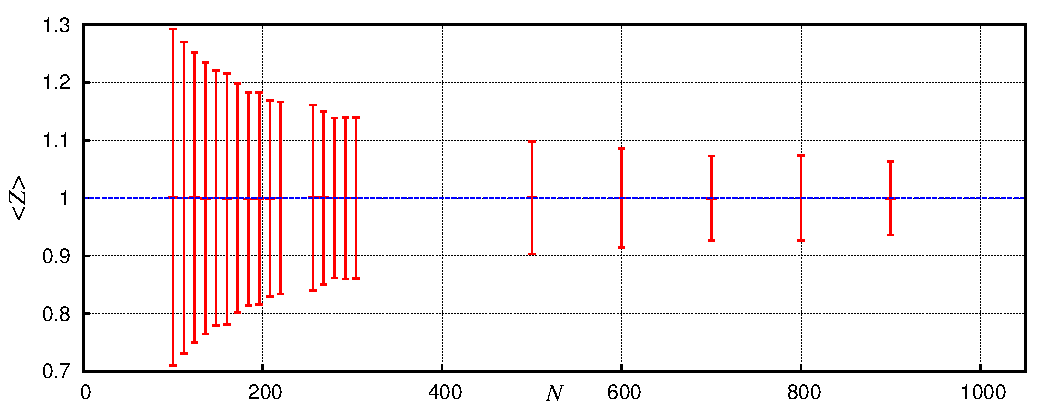
\includegraphics[scale=0.95]{Immagini/Soffici/ZvsN3D}
	\newline\footnotesize{ $d=3$ , campioni$= 500000$,  urti termal=$ 250000$, $\rho = 0.7$,	$E_D=-2.98$ per molecola}
	\label{fig: Limite Termo}
\end{figure}

Eseguendo un fit dei valori calcolato rispetto ad un andamento del tipo:
\begin{equation}\label{eq: limiteTermo}
 (Z-1) = A + \dfrac{B}{N}
\end{equation}
si ottengono le seguenti stime per i parametri della funzione:
\begin{center}
\begin{tabular}{|c c r c l |}
\hline
	A	 & $=$ & $ 2.98 $ & $\pm$ & $0.01 $	\\
	B	 & $=$ & $ 2.70$ & $\pm$ & $0.2 $	\\
\hline
\end{tabular}
\end{center}

Calcolando il limite per $N\rightarrow \infty$ si ottiene una stima del fattore di comprimibilità al limite termodinamico (a densità $\rho=0.7$ ed energia molecolare media $E_{mol} = -2.98$) pari a: 
\begin{displaymath}
Z_{\textrm{TD}} = 1 \pm 0.0001
\end{displaymath}

Un valore di Z pari ad 1 implica che il sistema in questo stato termodinamico soddisfa approsimativamente l'equazione di stato dei gas Perfetti:
\begin{displaymath}
 P V = n R T \rightarrow 1= \dfrac{P V}{n R T} =\dfrac{P \rho}{kT} = Z
\end{displaymath}
\newline \bigskip
Con lo stesso sistema è possibile studiare il limite termodinamico anche per gli altri osservabili del sistema.
Nella figura (\ref{fig: Limite Termo T}) è mostrato l'andamento di $T$ mentre nella figura (\ref{fig: Limite Termo U}) quello di $\frac{U}{N}$ espressi nelle unità dimensionali del modello e in funzione del numero di molecole $N$.
\begin{figure}[htbp]
\centering
	\caption[Sfere Soffici$/$Problema12.cpp $\quad \rightarrow \quad$ UvsN\_file.p]{Andamento dell'osservabile $\lbrace U/N \rbrace$ in funzione di $N$. Limite Termodinamico }\vspace{-15pt}
	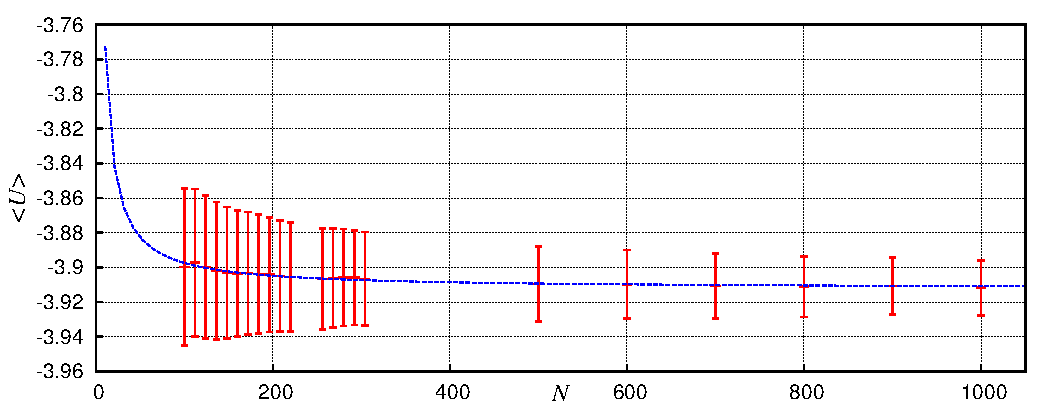
\includegraphics[scale=0.95]{Immagini/Soffici/UvsN3D}
	\newline\footnotesize{ $d=3$ , campioni$= 500000$,  urti termal=$ 250000$, $\rho = 0.7$,	$E_D=-2.98$ per molecola}	\label{fig: Limite Termo U}
\end{figure}
\begin{figure}[htbp]
\centering
	\caption[Sfere Soffici$/$Problema12.cpp $\quad \rightarrow \quad$ TvsN\_file.p]{Andamento del parametro $\lbrace T \rbrace$ in funzione di $N$. Limite Termodinamico }\vspace{-15pt}
	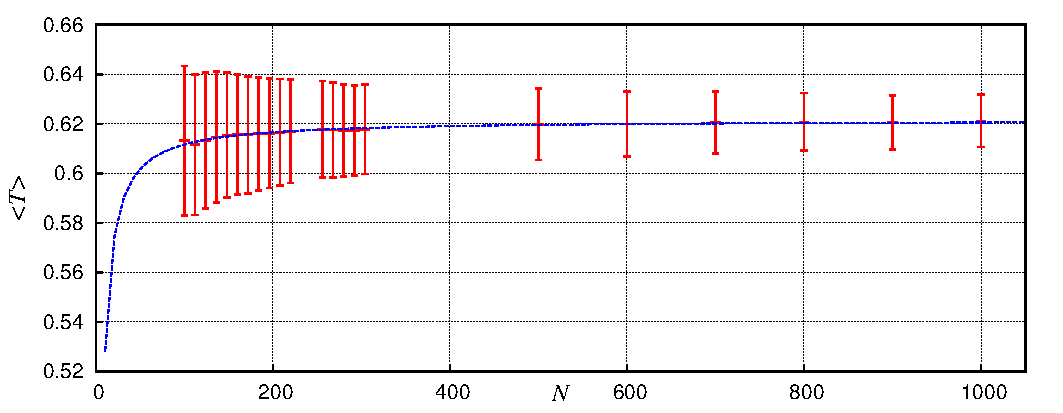
\includegraphics[scale=0.95]{Immagini/Soffici/TvsN3D}
	\newline\footnotesize{ $d=3$ , campioni$= 500000$,  urti termal=$ 250000$, $\rho = 0.7$,	$E_D=-2.98$ per molecola}	\label{fig: Limite Termo T}
\end{figure}
Usando per il fit di queste osservabili l'andamento precedente ( equazione \ref{eq: limiteTermo}) risulta la seguente stima per il limite termodinamico della temperatura e dell'energia interna:
\begin{displaymath}
T_{\textrm{TD}} = 0.6214 \pm 0.0003
\end{displaymath}
\begin{displaymath}
(U/N)_{\textrm{TD}} = -3.912 \pm 0.0005
\end{displaymath}
Si può osservare che i valori soddisfano la prescrizione di conservazione dell'energia meccanica totale:
\begin{displaymath}
\lbrace T \rbrace \dfrac{3}{2} + \lbrace U/N \rbrace =  0.931 - 3.912 = -2.98
\end{displaymath}